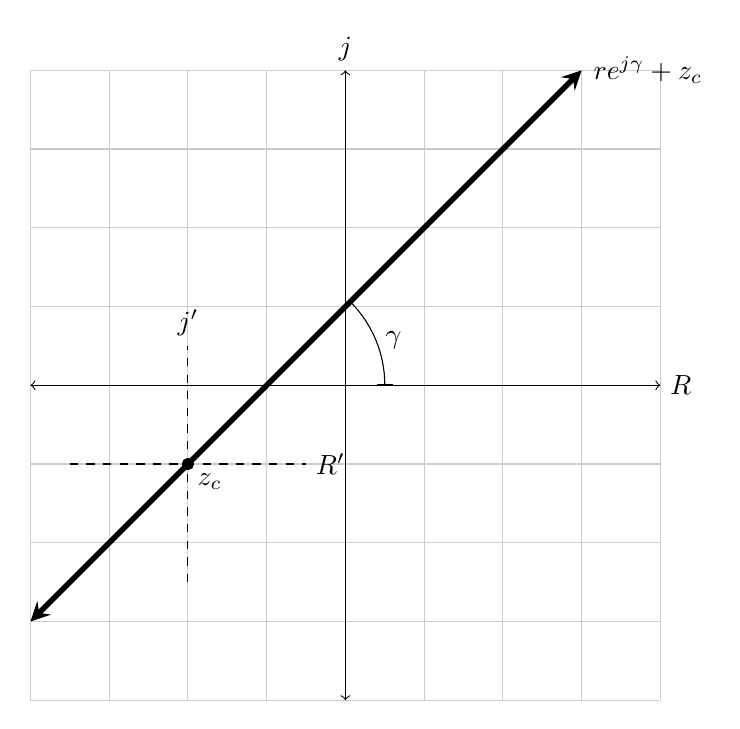
\begin{tikzpicture}
    \draw[thin,gray!40] (-4,-4) grid (4,4);
    \draw[<->] (-4,0)--(4,0) node[right] {$R$};
    \draw[<->] (0,-4)--(0,4) node[above]{$j$};
    \draw[dashed] (-3.5,-1)--(-0.5,-1) node[right] {$R'$};
    \draw[dashed] (-2,-2.5)--(-2,0.5) node[above]{$j'$};
    \draw [fill=black] (-2,-1) circle(2pt) node[anchor=north west]{$z_c$};
    \draw[line width=2pt,black,stealth-stealth] plot[smooth,domain=-4:3] (\x, {\x+1}) node[right]{$re^{j\gamma}+z_c$};
    \draw[|-|] (0.5,0) arc (0:45:1.5) node [midway, right]{$\gamma$};
\end{tikzpicture}
\caption{Recta genérica desplazada un $z_c$}